\section{Preliminary} \label{sec:prel}
In this section, the background of TMO ReRAMs are presented. Specifically, the resistance switching mechanisms of unipolar and bipolar ReRAM cell are introduced in detail. Then the cross-point architecture of ReRAM array is detailed.
\subsection{Metal Oxide Resistive Memory}
The resistance switching behavior is observed in many materials, such as
perovskite oxides, transition metal oxides, solid-state electrolytes, and organic materials. Among all of these materials, the TMO MIM structures attracted lots of research interests not only because its good electrical characteristics, such as fast access speed, high ON-OFF resistance ratio and low power consumption, but also because of is good scalability, 3-D stackability, as well as BEOL CMOS process capability.

A schematic view of the MIM structure of TMO based ReRAM cell is shown in Fig.~\ref{fig:overview}(a). The ReRAM cell has a very simple structure: a TMO based storage layer sandwiched by two metal layers of electrodes, named top electrode (TE) and bottom electrode (BE). As implied by its name, the ReRAM cell uses the resistance to represent the information stored in the cell: low resistive state (LRS or ON-state) and high resistive state (HRS or OFF-state) are used to represent the logic `1' and `0' respectively. As shown in Fig.~\ref{fig:overview}(a), in order to switch a ReRAM cell between the LRS and the HRS, a external voltage with specified polarity, magnitude, and duration is required. According to the switching behaviors, the ReRAM can be classified into two category: the bipolar and the unipolar ReRAM. For the unipolar ReRAM cell, the resistance switching only depends on the magnitude of the external voltage applied across the cell, independent of the polarity of the voltage. On the other hand, for the bipolar ReRAM cell, the LRS-to-HRS switching (aka RESET operation) and the HRS-to-LRS switching (aka SET operation) occur at different polarities.  In addition to SET and RESET operation, the forming operation is another important process for the ReRAM cell. Briefly, the forming operation is the first SET operation, which switch a fresh device into LRS by a soft dielectric breakdown. After the forming process, the device can be switched between LRS and HRS repeatedly. The demand of forming operations brings extra challenges and overheads to the ReRAM design since it always requires larger voltage/current than SET/RESET operation. Fortunately, researchers figured out that the forming voltage can be reduced linearly with the decrease of the thickness of the TMO thin film[cite]. Besides, the forming voltage can be also reduced by improving the deposition process[cite]. Recently, several forming-free ReRAMs have been proposed[][][]. The switching and forming mechanisms will be discussed in Section~\ref{sec:Model}. A variety of TMOs have already show the potential as the insulator layer of the MIM structure non-volatile ReRAM cell with different electrical characteristics such as operation voltage, switching speed, endurance, and retention time. Wong~\cite{review_wong} provided a comprehensive review of metal-oxide ReRAM with detailed discussion of HfOx, AlOx, NiO, TiOx, and TxOx based devices. However, in this paper, we will not focus on the different materials of the ReRAM cell. Conversely, we will study the general reliability issues, such as endurance failures and retention failures, that exist almost in all of the TMO based ReRAM.

\begin{figure}[!t]
\centering
    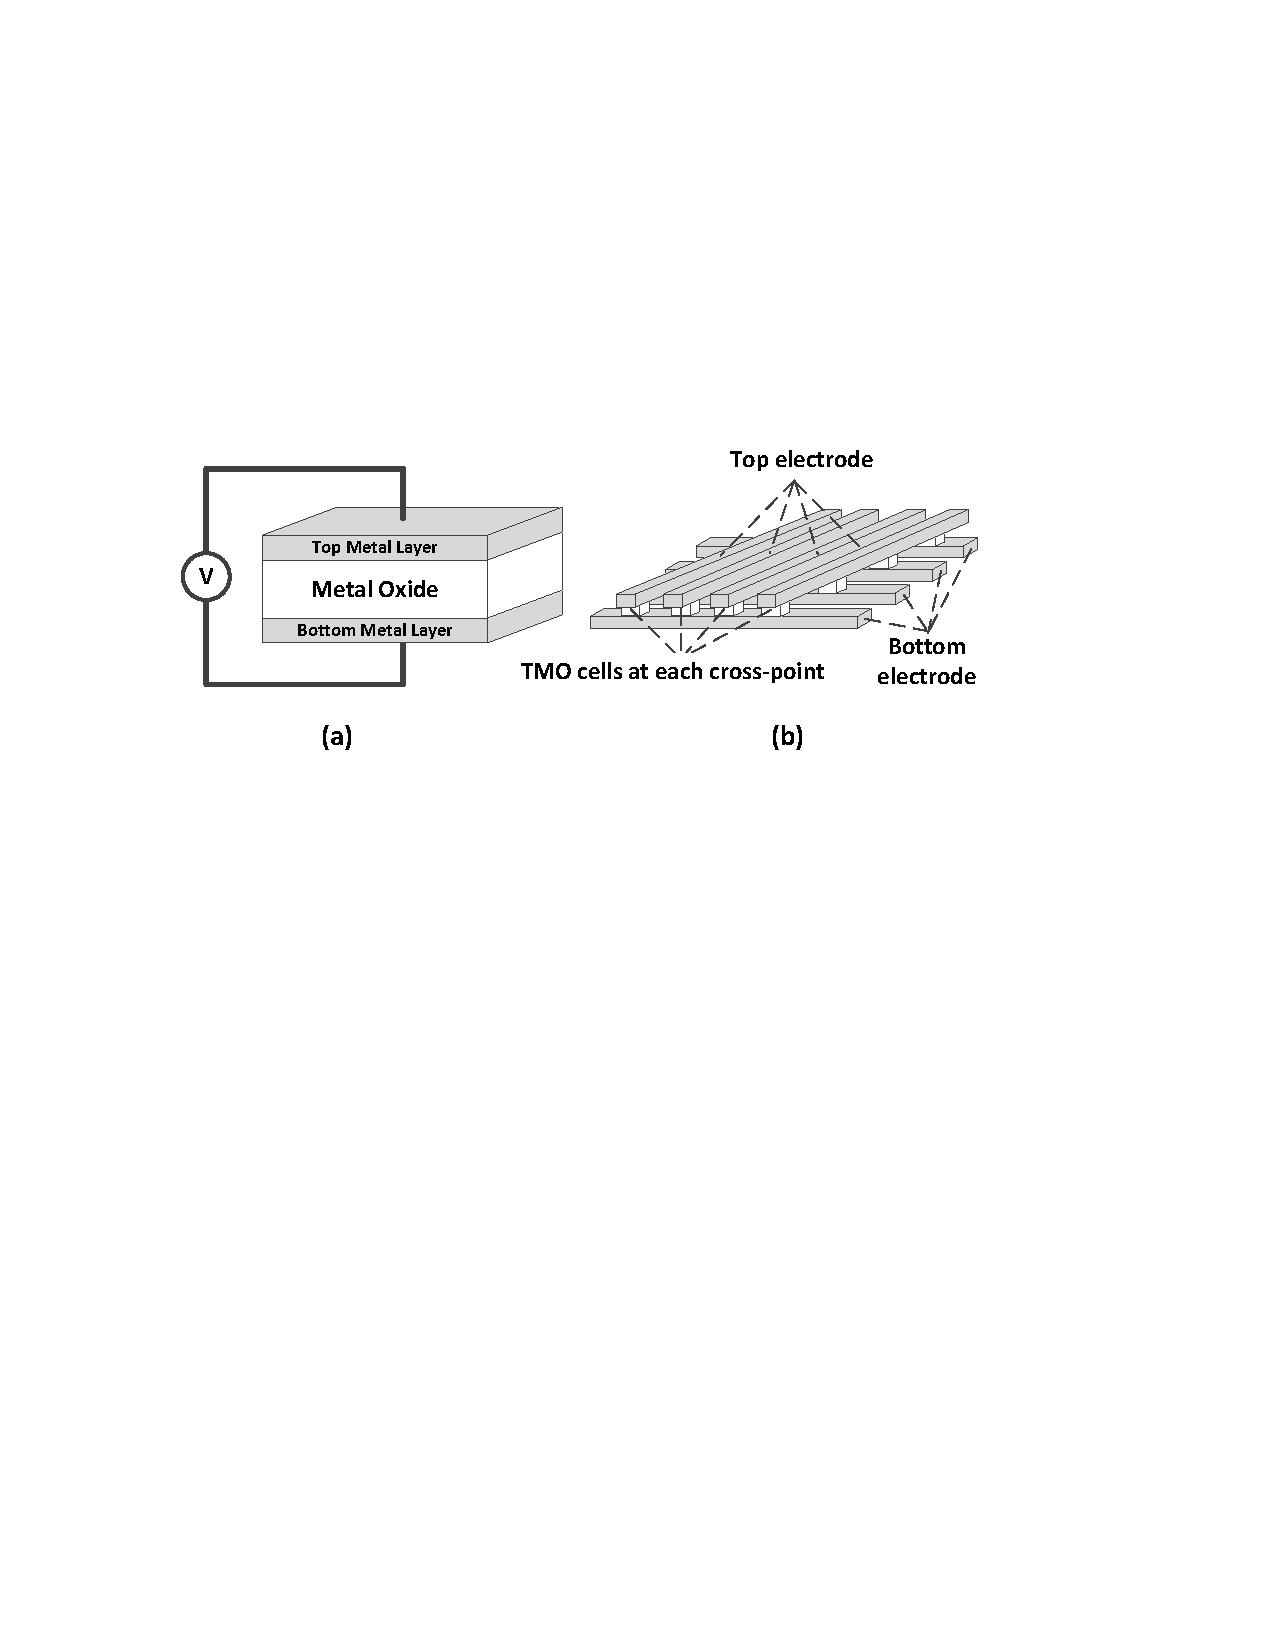
\includegraphics[width=3.3in]{./fig/DATE1.pdf}
\caption{An overview of (a) TMO MIM structure and (b) a cross-point ReRAM array.}
\label{fig:overview}
\end{figure}

